\section{Bug Detector}\label{sec:checker}

\begin{table}
  \centering
  \caption{Type-related specification bugs fixed by pull requests for the recent
  three years from 2018 to 2021.}
  \label{table:pr-bugs}
  \vspace*{-1.5em}
  \[
    \begin{array}{c|l|r|r}
      \multicolumn{1}{c|}{\textbf{Category}} &
      \multicolumn{1}{c|}{\textbf{Bug Kind}} &
      \multicolumn{1}{c|}{\textbf{\# PR}} &
      \multicolumn{1}{c}{\textbf{\# Bugs}}\\
      \hline

      \multirow{2}{*}{\stextsf{Reference}}
      & \stextsf{UnknownVar} & 5 & 12\\\cline{2-4}
      & \stextsf{DuplicatedVar} & 2 & 12\\\hline

      \multirow{1}{*}{\stextsf{Arity}}
      & \stextsf{MissParam} & 2 & 4\\\hline

      \multirow{1}{*}{\stextsf{Assertion}}
      & \stextsf{Assertion} & 4 & 5\\\hline

      \multirow{2}{*}{\stextsf{Operand}}
      & \stextsf{NoNumber} & 1 & 2\\\cline{2-4}
      & \stextsf{Abrupt} & 5 & 6\\\hline

      \multicolumn{2}{c|}{\textbf{Total}} & 19 & 41\\

    \end{array}
  \]
  \vspace*{-1.5em}
\end{table}

We develop a \textit{bug detector} to statically detect type-related
specification bugs in ECMAScript using an augmented abstract transfer
$\detector$ with additional checkers.  Before implementing checkers, we manually
investigated pull requests for the recent three years from 2018 to 2021 to get
insight of checkers.  As described in Table~\ref{table:pr-bugs}, there existed
19 pull requests that fixed 41 type-related specification bugs classified in
four categories and six kinds.  To detect such specification bugs, we implement
four checkers for four bug categories: a \textit{reference checker}, an
\textit{arity checker}, an \textit{assertion checker}, and an \textit{operand
checker}.  Now, we explain how each checker detects corresponding category of
bugs in the augmented abstract transfer $\detector$.


\subsection{Reference Checker}

In ECMAScript abstract algorithms, variables are dynamically introduced in any
contexts.  A \textit{reference bug} occurs when trying to access not yet defined
variables (\stextsf{UnknownVar}) or to redefine already defined variables
(\stextsf{DuplicatedVar}).  According to our manual investigation of pull
requests, the reference bug is the most prevalent type-related specification
bugs; 5 pull requests fixed 12 unknown variable bugs and 2 pull requests fixed
12 already defined variable bugs.  We implement the reference checker by adding
additional checks to abstract semantics of variable lookups and variable
declarations:
\begin{figure}[H]
  \centering
  \vspace*{-0.5em}
  \resizebox{\columnwidth}{!}{$
    \begin{array}{@{}l@{~}c@{~}l@{}}
      \aseme{\x}(\aenv) &=& \left\{
        \begin{array}{ll}
          \text{unknown variable} \; $\x$
          & \text{if} \; \asemr{\x}(\aenv) = \{ \tabsent \}\\
          \cdots
          & \text{otherwise}\\
        \end{array}
      \right.\\

      \asemi{\kwlet \; \x = \expr}(\lab, \tys)(\aelem) &=& \left\{
        \begin{array}{ll}
          \text{already defined variable} \; $\x$
          & \text{if} \; \aty = \{ \true \}\\
          \cdots
          & \text{otherwise}\\
        \end{array}
      \right.\\ &&
      \text{where} \; \aty = \aseme{\x \kwexists}(\aelem(\lab, \tys))\\
    \end{array}
  $}
  \vspace*{-0.5em}
\end{figure} \noindent
If the abstract semantics of a variable lookup for $\x$ is a singleton $\{
\tabsent \}$, $\x$ is always an unknown variable.  For example, consider the
syntax-directed algorithm at the upper-left in Figure~\ref{fig:example}.  Since
the \textbf{GetReferencedName} algorithm is removed, the variable
\code{GetReferencedName} does not exist in abstract environments and its lookup
returns $\{ \tabsent \}$ thus the reference checker reports the unknown variable
bug for \code{GetReferencedName}.  For already defined variables, the reference
checker utilizes the abstract semantics of existence check $\aseme{\x
\kwexists}$ to check whether the variable $\x$ of each variable declaration is
already defined.


\subsection{Arity Checker}

Arity of a function $\func = \kwdef \; \f (\p_1, \cdots, \p_n, \kwsl \cdots, p_m
\kwsr). \; \lab$ is defined as an interval $[n, m]$ where $n$ and $m-n$ denote
numbers of normal and optional parameters, respectively.  In function
invocations, \textit{missing parameters} (\stextsf{MissParam}) bugs occurs when
the number of arguments is not matched with the function arity.  In three years,
2 pull requests fixed 4 missing parameter bugs.  The arity checker detects such
missing parameters by using additional checks in the abstract semantics of
function call instructions:
\begin{figure}[H]
  \centering
  \vspace*{-0.5em}
  \resizebox{\columnwidth}{!}{$
    \begin{array}{@{}l@{}}
      \asemi{\x = \kwrl \expr \; \expr_1 \cdots \expr_k \kwrr}(\lab,
      \tys)(\aelem) =\\
      \qquad \left\{
        \begin{array}{ll}
          \text{missing parameters} \; \p_{k+1}, \cdots, \p_{n_\func} &
          \text{if} \; \exists \func \in \aty. \;\text{s.t.}\; k < n_\func\\

          \cdots &
          \text{otherwise}\\
        \end{array}
      \right.\\
      \qquad \text{where} \; \func = \kwdef \; \f (\p_1, \cdots, \p_{n_\func},
      \kwsl \cdots, p_{m_\func} \kwsr). \; \lab \;\wedge\;\\
      \qquad \phantom{\text{where}} \; \aty = \aseme{\expr}(\aelem(\lab,
      \tys)).\\
    \end{array}
  $}
  \vspace*{-0.5em}
\end{figure} \noindent
For each function $\func$ in the abstract semantics of the function expression
$\expr$, the arity checker compares the number of arguments with the arity of
$\func$ to detect missing parameters.  For example, consider the lower-left
syntax directed algorithm in Figure~\ref{fig:example}.  The algorithm invocation
in line 2 is compiled to a function call instruction:
\[
  \fcode{x = (formal.IteratorBindingInitialization formal)}
\]
with a temporal variable $\x$.  While it passes only a single argument
$\code{formal}$, the function arity is $[3, 3]$ thus the arity checker reports
missing parameter bugs for two additional parameters $\code{iteratorRecord}$ and
$\code{environment}$.


\subsection{Assertion Checker}
An \textit{assertion failure} (\stextsf{Assertion}) is a specification bug that
occurs when the condition of an assertion instruction is not true.  There
existed 4 pull requests that fixed 5 assertion failures.  The assertion checker
detects such bugs using additional checks in the abstract semantics of assertion
instructions:
\begin{figure}[H]
  \centering
  \vspace*{-0.5em}
  \resizebox{0.95\columnwidth}{!}{$
    \begin{array}{@{}l@{~}l@{}}
      \asemi{\kwassert \; \expr}(\lab, \tys)(\aelem) = & \left\{
        \begin{array}{ll}
          \text{assertion failure} \; \expr &
          \text{if} \; \{ \true \} \norder \aty\\

          \cdots &
          \text{otherwise}\\
        \end{array}
      \right.\\ &
      \text{where} \; \aty = \aseme{\expr}(\aelem(\lab, \tys))\\
    \end{array}
  $}
  \vspace*{-0.5em}
\end{figure} \noindent
It checks whether $\{ \true \}$ does not have partial order with the abstract
semantics of the condition expression $\expr$.  For example, consider the
lower-right syntax directed algorithm in Figure~\ref{fig:example}.  The
parameter $\code{environment}$ of this algorithm has an environment record or
$\undefval$.  Since type sensitivity divides the abstract types of arguments to
upcasted single types, there are two different abstract environments whose
variable $\code{environment}$ points to $\{ \code{Environment} \}$ or $\{
\undefval \}$.  When $\code{environment}$ is $\{ \code{Environment} \}$, the
abstract semantics of assertion condition $\code{environment = originalEnv}$ is
$\{ \tbool \}$.  Even though we know that the type of $\code{originalEnv}$ is
also $\{ \code{Environment} \}$, \code{Environment} is not a singleton type thus
we cannot convince that they are the exactly same environment.  Thus, we cannot
say that the assertion must be failed in this case.  However, if
$\code{environment}$ is $\{ \undefval \}$, the abstract semantics of the
condition $\code{environment = originalEnv}$ is $\{ \false \}$ because an
environment is never equal to $\undefval$.  Thus, the assertion checker reports
an assertion failure for the condition $\code{environment = originalEnv}$.


\subsection{Operand Checker}

\begin{figure*}
  \centering
  \begin{subfigure}[b]{0.24\textwidth}
    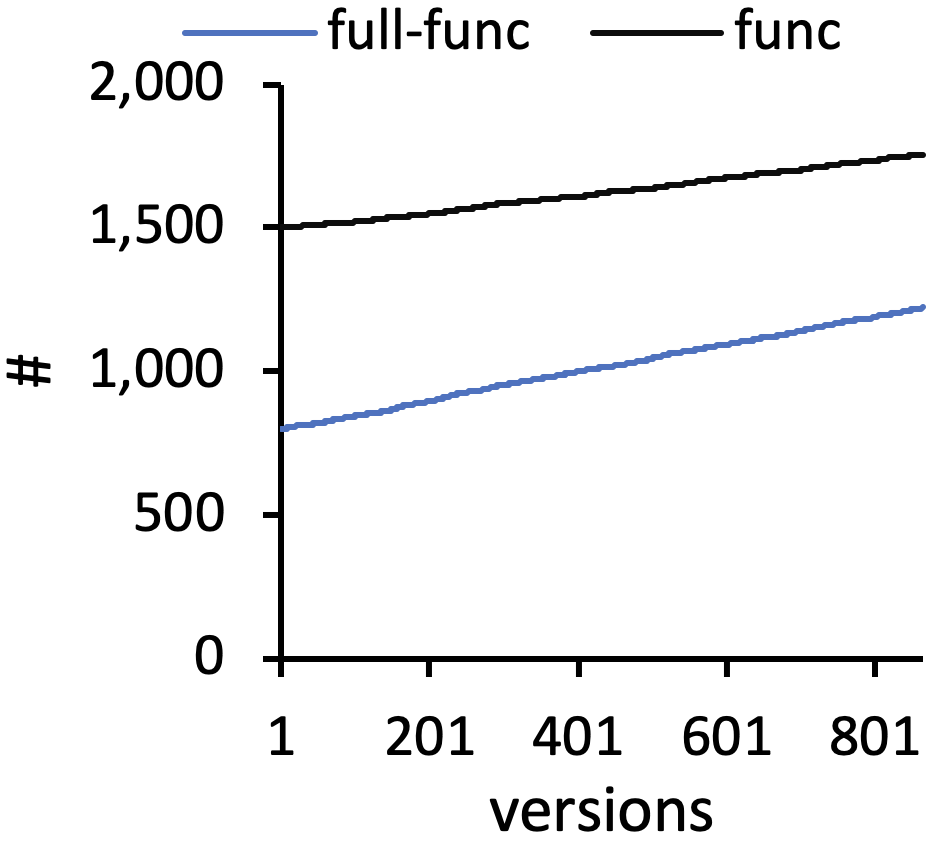
\includegraphics[width=\textwidth]{img/func}
    \caption{The number of functions.}
  \end{subfigure}
  \begin{subfigure}[b]{0.24\textwidth}
    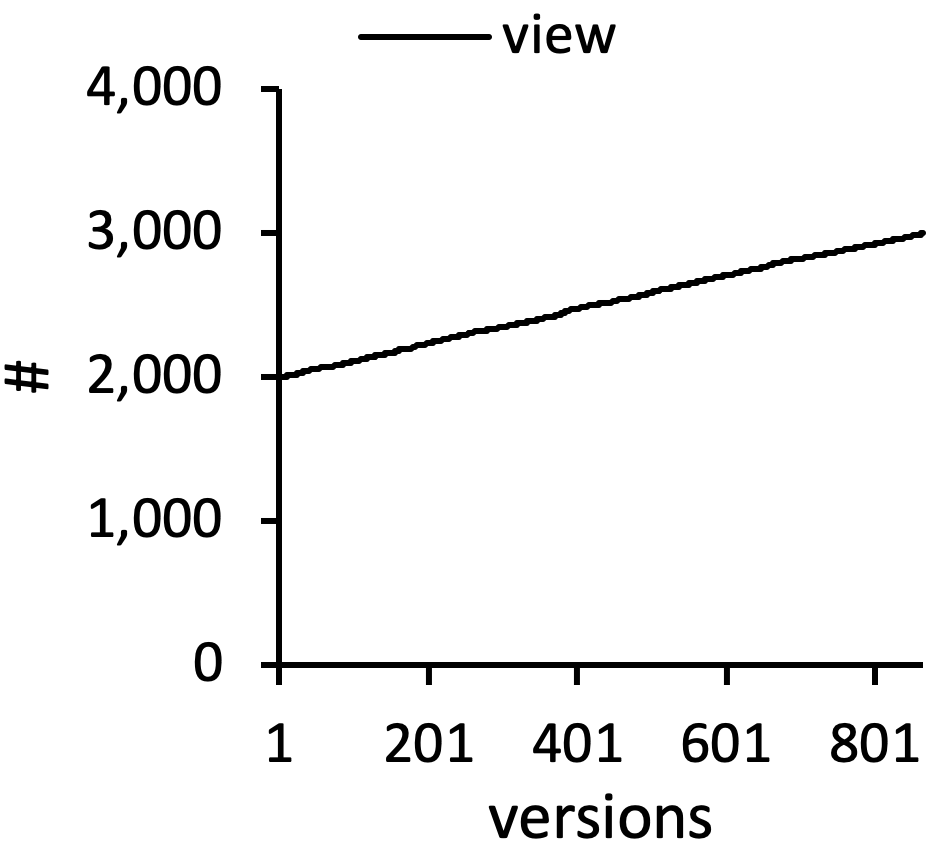
\includegraphics[width=\textwidth]{img/view}
    \caption{The number of views.}
  \end{subfigure}
  \begin{subfigure}[b]{0.24\textwidth}
    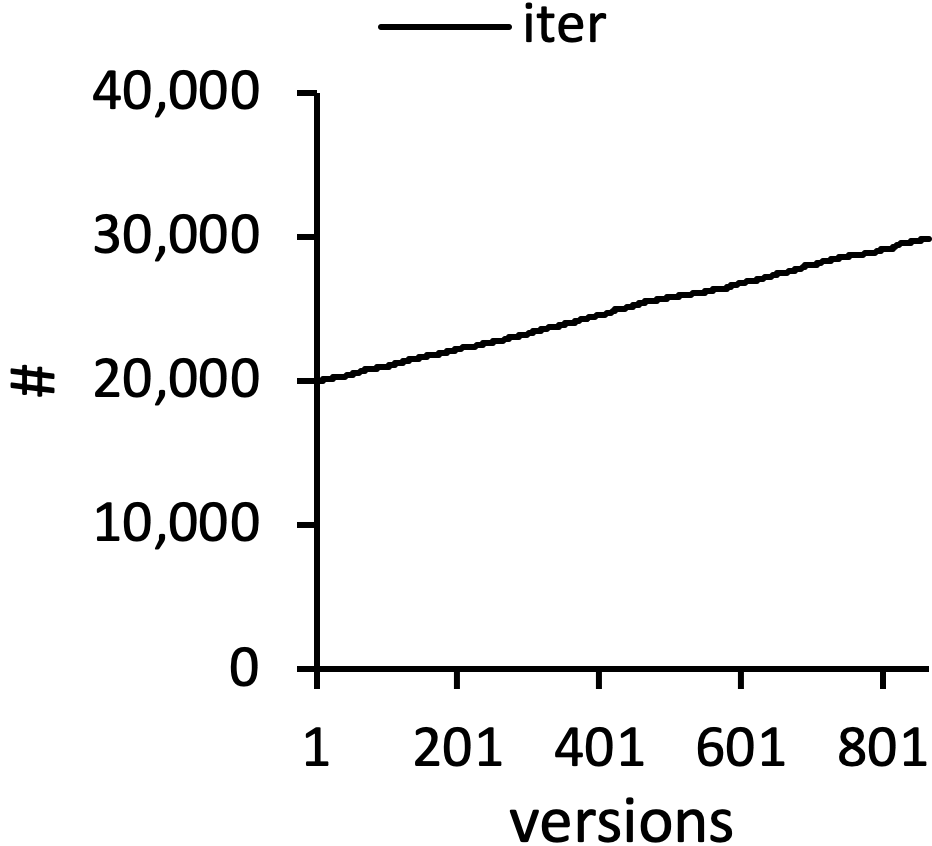
\includegraphics[width=\textwidth]{img/iter}
    \caption{The number of iterations.}
  \end{subfigure}
  \begin{subfigure}[b]{0.24\textwidth}
    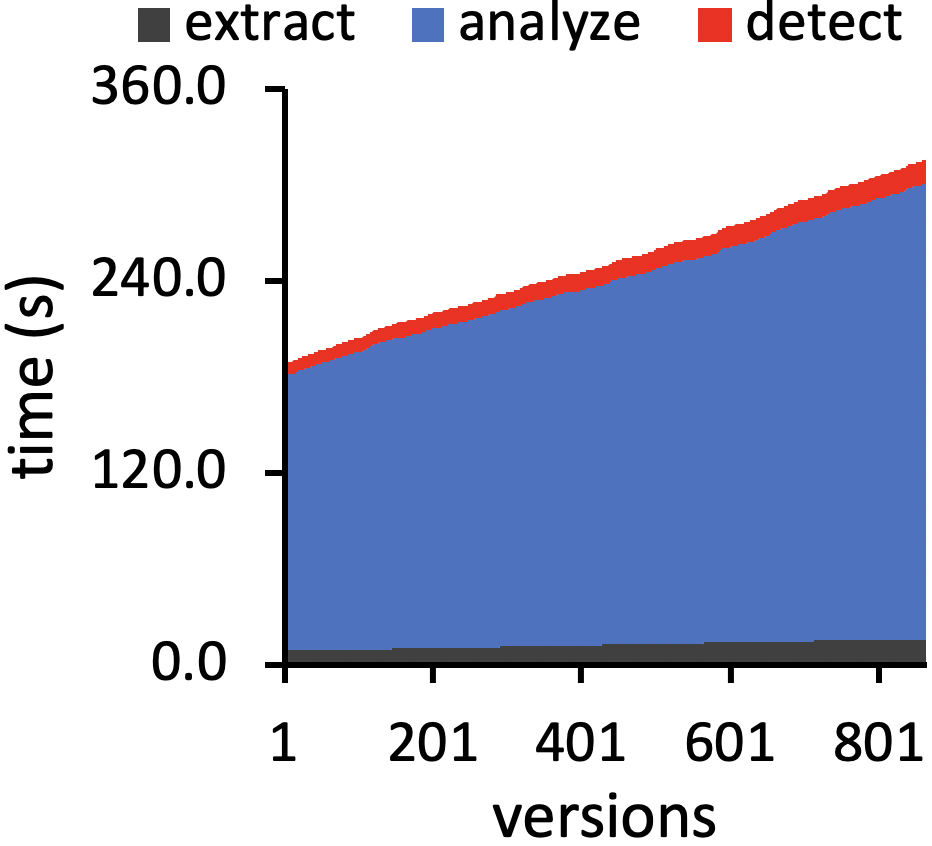
\includegraphics[width=\textwidth]{img/time}
    \caption{The analysis time.}
  \end{subfigure}
  \caption{The statistics of type analysis using $\tool$ for 864 versions of
  ECMAScript.}
  \vspace*{-1.5em}
  \label{fig:stat}
\end{figure*}

Several operators are typed and a \textit{ill-typed operand bug} occurs when
the type of an operand is not conform to the expected type.  For example, the
comparison operator $\code{<}$ is a numeric operator in the modified $\ires$.
If an expression tries to compare between non-numeric values such as $\true <
\code{"abc"}$, then it is a non-numeric operand bug (\stextsf{NoNumber}).
Besides, ECMAScript has a special implicit conversion for normal completions
when their actual values stored in the $\code{Value}$ field are required
including conditions, values of field updates, operands of operators, etc.  For
example, if the variable $\x$ has a normal completion with \code{42} as its
actual value, $\code{x + 1}$ should \code{43} because the normal completion
implicitly converted into its actual value \code{42}.  To explicitly represent
this conversion, let's define a unary operator $\escaped$:
\begin{figure}[H]
  \centering
  \vspace*{-0.5em}
  \resizebox{\columnwidth}{!}{$
    \escaped \val = \left\{
      \begin{array}{ll}
        \val &
        \text{if} \; \val \; \text{is not a completion}\\

        \val.\code{Value} &
        \text{if} \; \val \; \text{is normal}\\

        \text{unchecked abrupt completion} \; \val &
        \text{otherwise}\\
      \end{array}
    \right.
  $}
  \vspace*{-0.5em}
\end{figure} \noindent
and assume that the operator $\escaped$ is used when the actual value is
required.  Then, an unchecked abrupt completion bug (\stextsf{Abrupt}) occurs
when the actual value is required but it is an abrupt completion.  According to
our manual investigation, 1 pull request is related to 2 non-numeric operand
bugs and 5 pull requests are related to 6 unchecked abrupt completion bugs.

The operand checker detects such ill-typed operand bugs by using additional
checks in the abstract semantics of binary operations and unary operations:
\begin{figure}[H]
  \centering
  \vspace*{-0.5em}
  \resizebox{0.9\columnwidth}{!}{$
    \begin{array}{@{}l@{~}c@{~}l@{}}
      \aseme{\expr_0 \bop \expr_1}(\aenv) &=& \left\{
        \begin{array}{ll}
          \text{ill-typed operand} \; \expr_0
          & \text{if} \; \asemr{\expr_0}(\aenv) \norder \aty_0\\
          \text{ill-typed operand} \; \expr_1
          & \text{if} \; \asemr{\expr_1}(\aenv) \norder \aty_1\\
          \cdots
          & \text{otherwise}\\
        \end{array}
      \right.\\

      \aseme{\uop \; \expr}(\aenv) &=& \left\{
        \begin{array}{ll}
          \text{ill-typed operand} \; $\expr$
          & \text{if} \; \asemr{\expr}(\aenv) \norder \aty\\
          \cdots
          & \text{otherwise}\\
        \end{array}
      \right.\\
    \end{array}
  $}
  \vspace*{-0.5em}
\end{figure} \noindent
where $\aty_0$, $\aty_1$, and $\aty$ are expected abstract types of $\expr_0$,
$\expr_1$, and $\expr$, respectively.  The additional check reports when the
given operand does not conform to the expected types.  For example, consider the
upper-right built-in algorithm $\code{Math.round}$ in Figure~\ref{fig:example}.
The parameter $\x$ has $\{ \tjs \}$ and $\n$ has $\{ \tnum \}$ because the
\textbf{ToNumber} algorithm always return number values or abrupt completions
but later cases are removed by the \textbf{ReturnIfAbrupt} prefix ?.  While the
built-in algorithm correctly uses $\n$ in line 2, it misuses $\x$ in line 3 and
4 and $\{ \tjs \}$ does not have a partial order with the expected abstract type
$\{ \tnum, \tbigint \}$.  Thus, the operand type checker reports non-numeric
operand bugs.
